\documentclass[a4paper,ngerman]{scrartcl}

\usepackage[utf8]{inputenc}
\usepackage{amssymb}

\usepackage[ngerman]{babel}
\usepackage{pdfpages}

\usepackage{graphicx}

\usepackage[protrusion=true,expansion=true]{microtype}

\usepackage{hyperref}
\usepackage{lmodern}
\usepackage{tabto}

\setlength\parskip{\medskipamount}
\setlength\parindent{0pt}

\usepackage{geometry}
\geometry{tmargin=1.5cm,bmargin=2cm,lmargin=1.5cm,rmargin=1.5cm}

\pagestyle{empty}

\setlength{\fboxrule}{2pt}
\setlength{\fboxsep}{-3pt}

\newcommand{\drawHere}{%
  \begin{center}%
    \fbox{\parbox[c][0.9\textwidth]{0.9\textwidth}{\ }}%
  \end{center}}

\newcommand{\header}{%
  \begin{raggedleft}
  \tiny Universität Augsburg \\
  Tag der Mathematik 2014 \par
  \end{raggedleft}}

\begin{document}

\header

\begin{center}
  \Huge\bf
  Das Möbiusband
\end{center}

\vspace{8 mm}
\begin{center}
    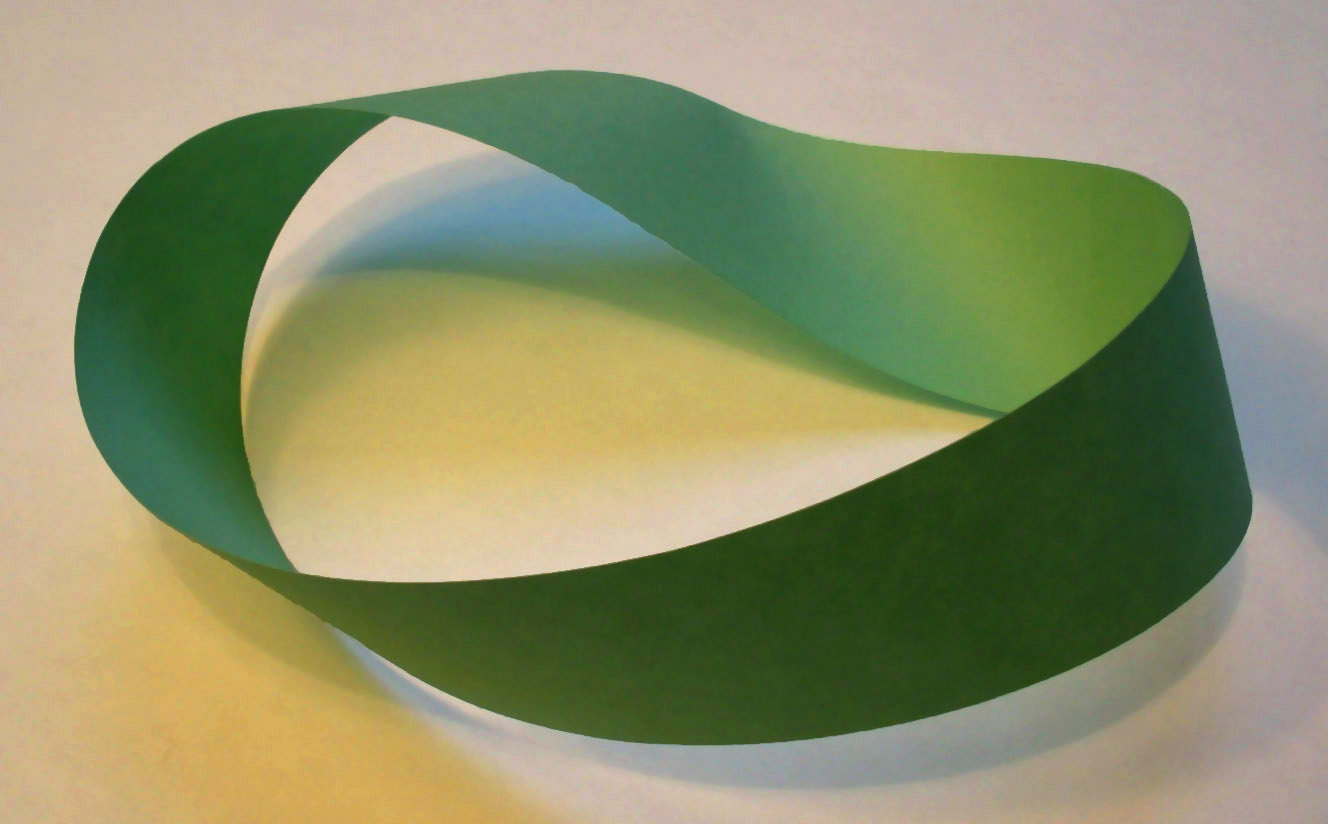
\includegraphics[scale=0.25]{moebiusband.jpeg}
\end{center}

\renewcommand{\labelitemi}{$\infty$}

\vspace{10 mm}
\Large
\begin{itemize}
  \item Ein \emph{Möbiusband} erhält man, wenn man einen Papierstreifen einmal
  verdrillt und dann an den Enden zusammenklebt.

  \item Das wunderliche am Möbiusband ist, dass es \emph{nur eine Seite} hat!
  Fahre mit einem Stift das Möbiusband ab. Du wirst feststellen, dass du
  \emph{ohne abzusetzen} das ganze Band bemalt haben wirst.
  
  \item Wie viele Ränder besitzt das Möbiusband? Um das herauszufinden, fahre
  mit einem Stift die Kante des Möbiusbands ab.

  \item Bastele ein normales Band und zerschneide es längs der Mitte. Was
  passiert?
  
  Wenn man dasselbe mit einem Möbiusband macht, passiert etwas ganz anderes.
  Was? Probiere es aus!

  \item Bastele zwei normale Bänder und klebe sie an den Klebestellen senkrecht
  aufeinander. Zerschneide die Bänder dann längs der Mitte: zuerst das eine,
  dann das andere. Was passiert?

  \item Bastele zwei Möbiusbänder, aber eines davon spiegelverkehrt --
  verdrille das eine also anders herum als das andere, bevor du die Enden
  zusammenklebst. Klebe die beiden Bänder dann an den Klebestellen senkrecht
  aufeinander. Zerschneide nun die beiden Bänder längs der Mitte: zuerst das
  eine, dann das andere. Dann passiert etwas völlig wunderliches. Was?

  \item Informiere dich bei Wikipedia über die Anwendungen von Möbiusbändern in
  der Technik!
\end{itemize}

\newpage


\header

\begin{center}
  \Huge\bf
  Die Kochsche Schneeflocke
\end{center}

\vfill
\drawHere

\vfill
\Large

\renewcommand{\labelitemi}{$\bigstar$}

\begin{itemize}
  \item So konstruiert man die Kochsche Schneeflocke:

  \begin{center}
    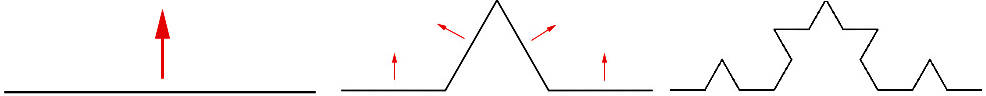
\includegraphics[scale=0.5]{koch}
  \end{center}
  \item Was ist ihr Umfang?
  \item Was ist ihr Flächeninhalt?
\end{itemize}

\newpage


\header

\begin{center}
  \Huge\bf
  Das Sierpinski-Dreieck
\end{center}

\vfill
\drawHere

\vfill
\Large

\renewcommand{\labelitemi}{$\blacktriangle$}

\begin{itemize}
  \item Spiele folgendes \emph{Chaosspiel}:
  \begin{enumerate}
    \item Zeichne ein großes gleichseitiges Dreieck.
    \item Wähle einen beliebigen Startpunkt im Dreieck.
    \item Such dir zufällig eine der drei Ecken aus.
    \item Markiere als neuen Punkt die Mitte zwischen deiner gewählten Ecke und \\ dem
    vorherigen Punkt.
    \item Fahre mit dem neuen Punkt bei Schritt 3 fort.
  \end{enumerate}
\end{itemize}

\enlargethispage{3em}
\begin{minipage}{0.9\textwidth}

\begin{itemize}
  \item Obwohl man den Startpunkt und die Ecken völlig zufällig wählt, ergibt
  sich erstaunlicherweise näherungsweise eine regelmäßige Figur: das \emph{Sierpinski-Dreieck}.
  \item Deterministisch (ohne Zufall) kann man es auch so konstruieren:

  \begin{center}
    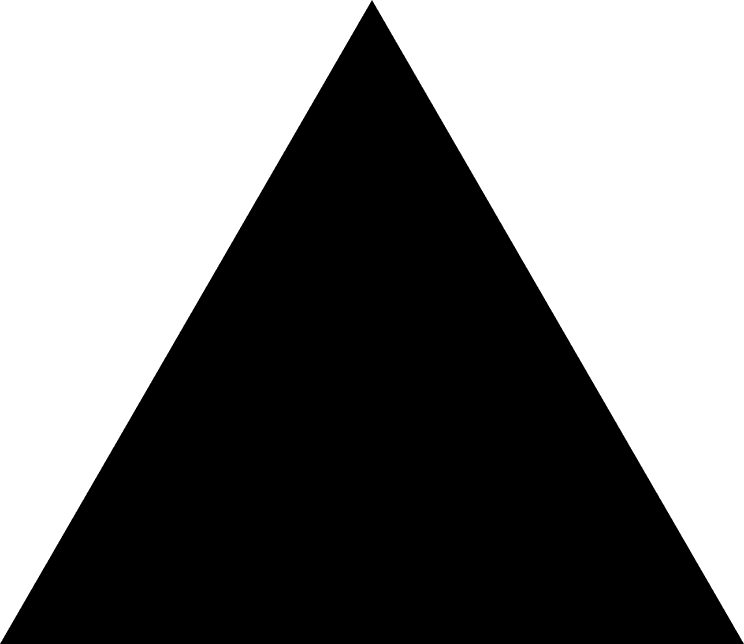
\includegraphics[scale=0.1]{sierpinski-1}\hfill
    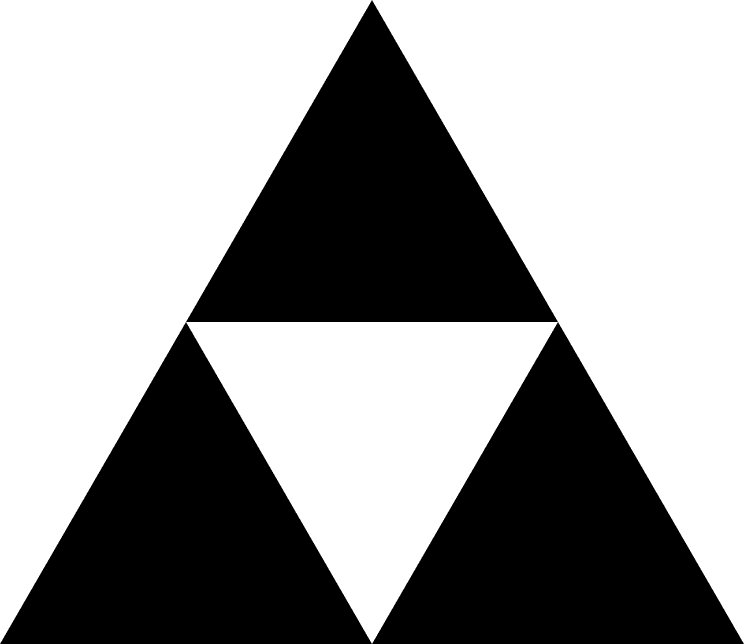
\includegraphics[scale=0.1]{sierpinski-2}\hfill
    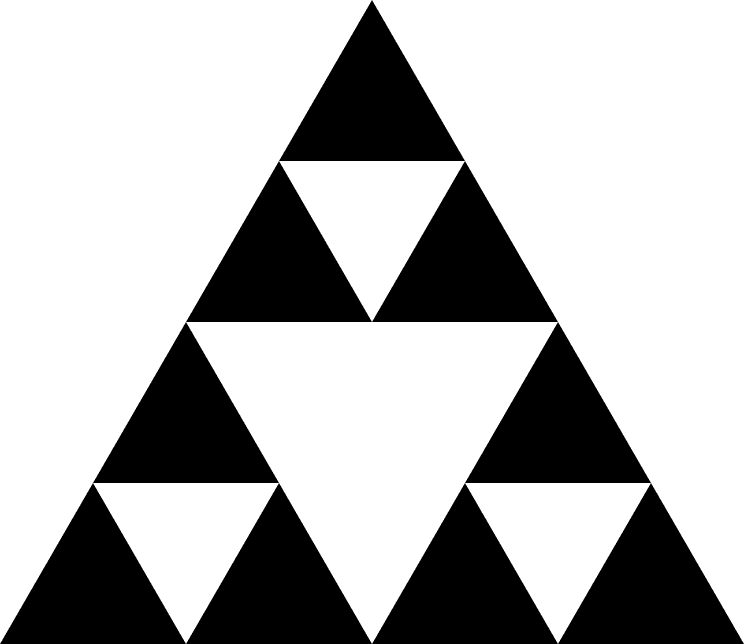
\includegraphics[scale=0.1]{sierpinski-3}\hfill
    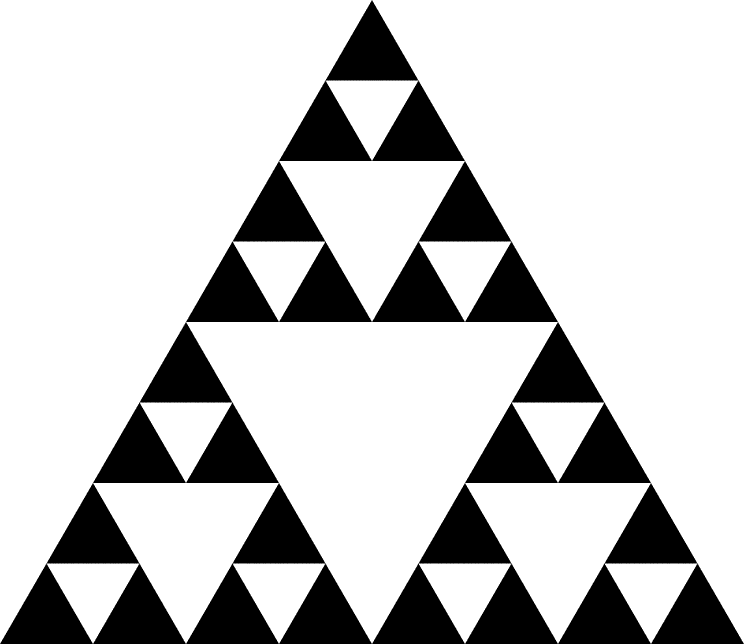
\includegraphics[scale=0.1]{sierpinski-4}
  \end{center}
  \item Wieso ergibt sich beim Chaosspiel dieses Sierpinski-Dreieck?

  Der Abstand der Punkte beim Chaosspiel zum tatsächlichen, völlig regelmäßigen
  Sierpinski-Dreieck halbiert sich mit jedem Schritt. Für das bloße Auge liegen
  daher alle Punkte (bis auf einige wenige zu Beginn) auf dem
  Sierpinski-Dreieck. Durch die zufällige Eckenwahl wird das ganze Dreieck
  gleichmäßig gefüllt.
  
  \begin{center}
    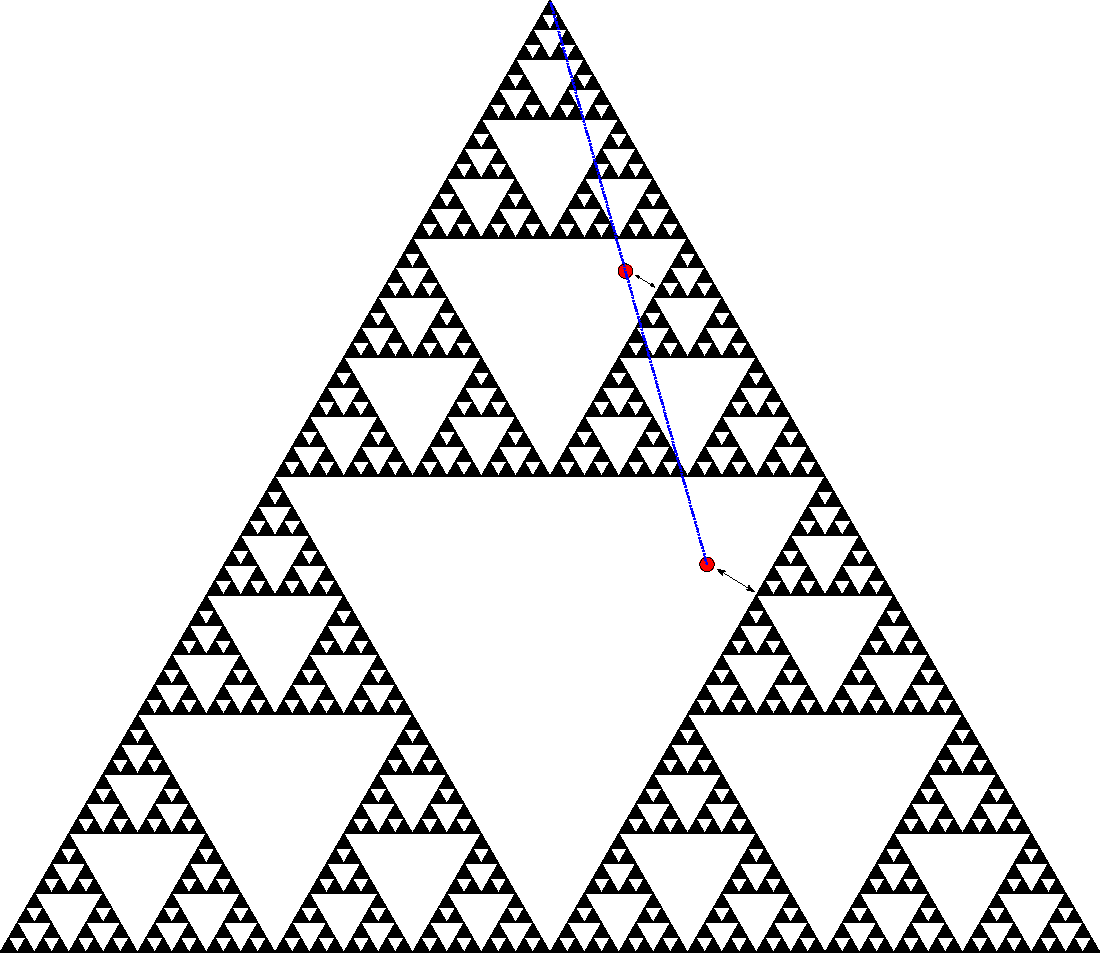
\includegraphics[scale=0.45]{sierpinski-beweis}
  \end{center}
  \item Was ist der Umfang des Sierpinski-Dreiecks?
  \item Was ist der Flächeninhalt des Sierpinski-Dreiecks?
  \item Die Kochsche Schneeflocke und das Sierpinski-Dreieck sind Beispiele für
  sog. \emph{Fraktale} (von lateinisch \emph{fractus}, "`gebrochen"').
  Annäherungen an Fraktale findet man an vielen Stellen in der Natur,
  etwa beim Romanesco-Blumenkohl, bei Flusssystemen, beim Blutkreislauf und bei
  Küstenlinien; außerdem sind manche physikalische Diagramme von fraktaler
  Natur.

  Fraktale sind
  wichtig, um sich klarzumachen, wie wunderlich geometrische Figuren sein
  können, und haben auch noch einen praktischen Nutzen: Fraktale werden
  in der Computergrafik eingesetzt, um realistisch aussehende Wälder und
  Wolken automatisiert
  generieren zu können.
\end{itemize}

\end{minipage}

\vfill
\hfill\small Chaosspiel direkt auf \url{http://tiny.cc/chaosspiel} spielbar

\end{document}
